 \documentclass{article}
\usepackage{cite}
\usepackage{inputenc}
\usepackage{setspace}
\usepackage[margin=0.75in]{geometry}
\usepackage[style=numeric]{biblatex}
\addbibresource{../bibs/ref.bib}
\usepackage{float}
\usepackage{graphicx}
\graphicspath{ {./images/} }


\onehalfspace
\setlength{\parindent}{0pt}
\setlength{\parskip}{1em}



\begin{document}

\begin{center}
  \LARGE{\textbf{Real-world Functional Programming}} \\
  \Large{Coursework Part I Report} \\
  \normalsize{14274056 Junsong Yang (psyjy3)} \\
  \today
\end{center}


\begin{normalsize}
  \section{Task I.1}
  The key ideas for this task are to explore the infinite data structure
  in haskell and to gain a better understanding of lazy evaluation in haskell.

  \begin{figure}[H]

    \begin{minipage}[b]{0.48\linewidth}
      \centering
      \centerline{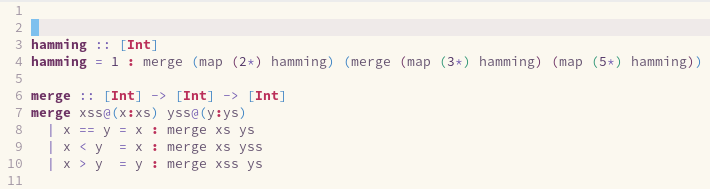
\includegraphics[width=8.0cm]{Hamming}}
      % \vspace{1.5cm}
      \centerline{ (a) Hamming Function Definition}\medskip
    \end{minipage}
    \hfill
    \begin{minipage}[b]{0.48\linewidth}
      \centering
      \centerline{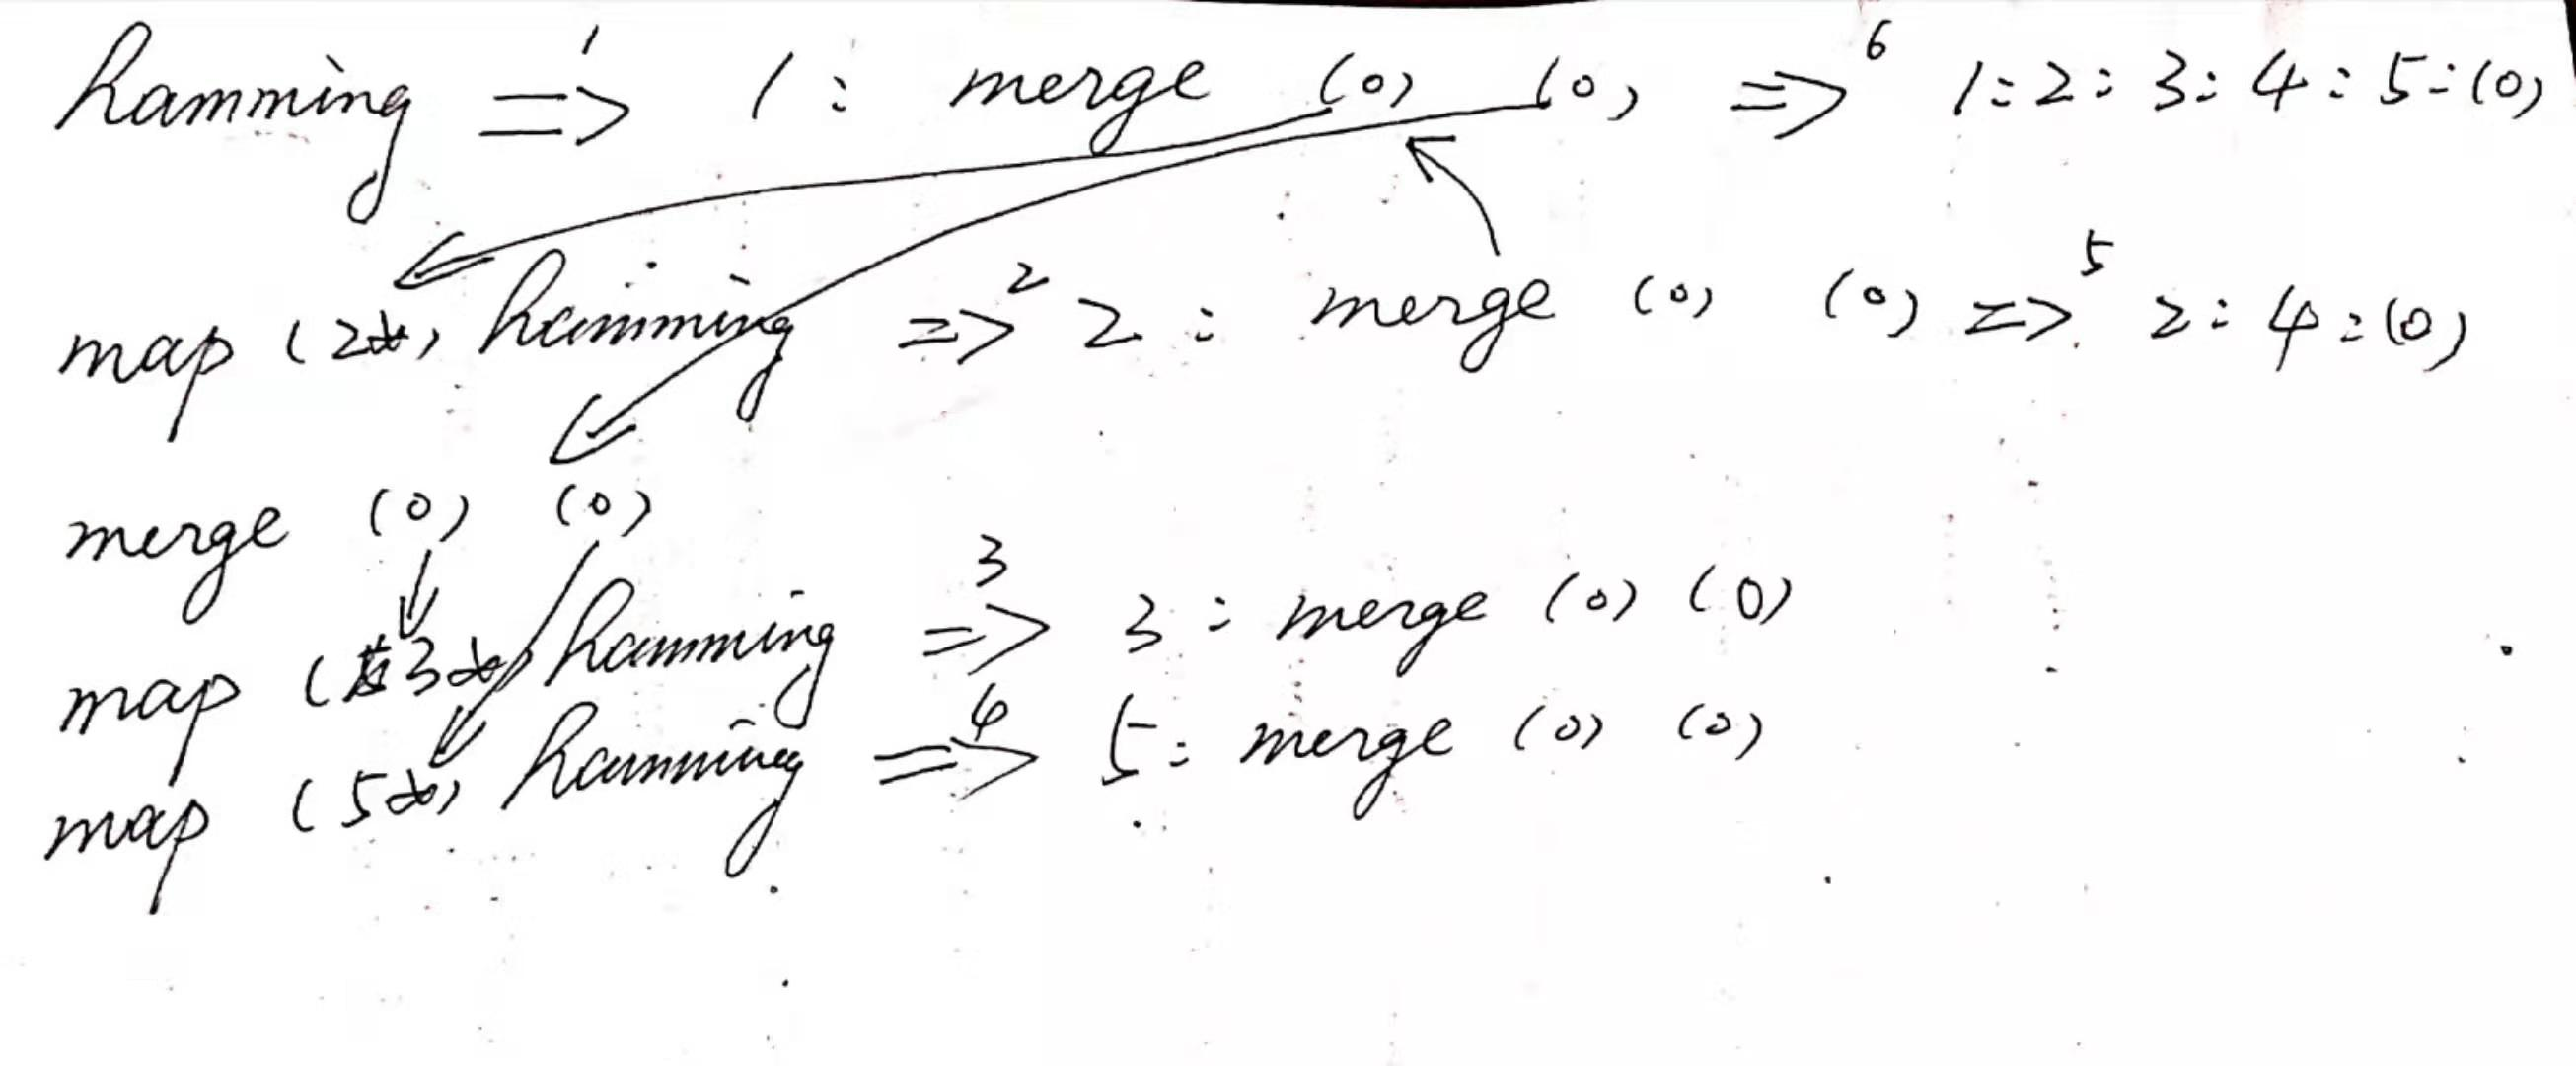
\includegraphics[width=8.0cm]{cyclic}}
      % \vspace{1.5cm}
      \centerline{ (b) Cyclic Graph}\medskip
    \end{minipage}
    % 
    \caption{TaskI.1}
    \label{fig:taskI.1}
    % 
  \end{figure}


  Hence, the hamming function can be defined as a infinite list in a recursive
  manner. As Figure \ref{fig:taskI.1} (a) shows, the type of hamming function is
  a list of Int. This implementation using map function to calculate 2x, 3x and
  5x and then merge then together as Figure \ref{fig:taskI.1} (b) demonstrated
  how it was evaluated.

  \section{Task I.2}
  The key ideas of this task are extend the current function to caculate sums
  and averages of range of cells and to explore the weakness of this evaluator
  then provide a solution.

  \begin{figure}[H]
    \centering
    \centerline{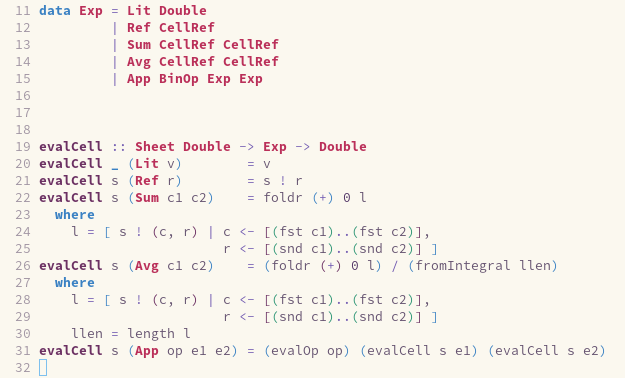
\includegraphics[scale=0.5]{Sheet}}
    \caption{Extended Evaluator}
    \label{fig:sheet}
  \end{figure}

  Figure \ref{fig:sheet} demostrates how evalCell function was extended to
  support Sum and Avg expression. The key idea of this implemetation is to given
  to CellRef c1 and c2, find every cell in between. Next, lookup corresponding
  values in the given sheet s. Then put all the values found in sheet s in list
  l. Finally using foldr to calculate the sum of all values.

  The similiar idea was used to implemetate the evaluation of Avg expression but
  a further step was taken to yield the average value.

  The most obvious weakness of this evaluator is that it will stuck in infinite
  loop when there are cyclic references in the given sheet. As the type
  signature indicates, the evalCell function will return a Double for every
  given sheet s and an Exp

  

  \section{Task I.3}

  \section{Task I.4}

  \section{Task I.5}



\end{document}


